\chapter{\label{ethnographicSetting}Ethnographic Setting}

\section{Introduction}
Having established a theory of social bonding through joint action, mediated by cognitive mechanisms recognisable in the phenomenon of team click, it is important to consider how this theory can be applied to specific real-world instances of joint action. There is considerable variation in the nature and dynamics of joint action, even within the sub-category of group exercise. Joint action in group exercise ranges from tightly coupled dyadic or group activities such as rowing, synchronised diving, or dance sport, to interactive competitive team sports like basketball, ice hockey, and rugby, through to more loosely coupled (but still time- and space-coordinated) mass participation activities such as marathons and triathlons.  It is sensible to assume that, as the scale and requirements of these contexts vary, so too will the psychophysiological mechanisms most responsible for enabling successful joint action, feelings of team click, and social bonding \citep{Mogan2017,Launay2016}.

Interactive and co-active team sports in particular contain dimensions of complexity that are not directly addressed by the existing experimental literature concerning joint action.  The competitive nature of these sporting practices means that co-actors in joint action scenarios will perform roles that either facilitate or inhibit shared goal achievement, depending on their team assignment \citep{Renshaw2009}. Competitive joint action appears to facilitate two modes of communication between individual participants: more predictable behaviour between cooperators and less-predictable action behaviour between opponents \citep{Glover2017}. The competitive dimension of interactive team sports thus introduces a complexity whereby subunits of cooperating co-actors coordinate their behaviours around a shared goal (winning the specific contest) \citep{Passos2012}, while at the same time, co-actors from both teams coordinate with each other around the higher order shared goal of completing a competitive game.
In addition, interactive team sports involve the nesting of coordinated subunits of actors and sub-phases of actions \citep{Vilar2012}.  For example, a dyadic joint action such as passing a ball between two attacking players in football is nested in a larger attacking sub-phase the defending team's goal in order to score a goal, which in turn is nested within a larger shared goal of beating the opposing team in a 90 minute match, and so on.  These dimensions of complexity in interactive team sports increase the overall degrees of freedom (i.e., ``free energy'') of joint action tasks, thus demanding higher technical competence from athletes in order to successfully establish functional interpersonal synergies capable of reducing such uncertainty \citep{Duarte2012}.

In addition to micro-level details and dynamics of joint action, macro-level variation in the cultural contexts of joint action also vary extensively.  As sporting anecdote indicates, different teams from different places and times appear to play the same game in very different ways---embodying different ``styles'' of play.  While there is very little literature devoted to examining the effect of cultural variation on joint action and social bonding in particular, there is extensive evidence to suggest that cultural variation impacts on processes of cognition \citep{Nisbett2003,Hoshino-Browne2005}, social learning \citep{Mesoudi2015}, and prosocial behaviour \citep{Yuki2005,Yuki2003}.  This suggests that cultural environments structure joint action scenarios in ways that help ``smooth'' coordination by providing equivalent expectations between co-participants \citep{Vesper2017}.
It is also important to bear in mind that, while the neurological, cognitive, and psychological theories from which the predictions of this dissertation strive for universal generalisability, these theories are nonetheless heavily grounded in Western epistemological assumptions, intuitions, and ``WEIRD'' empirical evidence \citep{Henrich2010a}. As such, it is important to consider, first, the ways in which these theories could direct attention towards certain empirical details over others. Second, it is crucial to consider how psychological theories joint action and social bonding can be advanced and developed.  In the next section, I outline my specific area of study in order to set the foundation for three empirical studies into the relationship between joint action and social bonding.

\section{Overview of research}
The empirical content of this dissertation is drawn from on one contemporary instance of group exercise, in one geographic region.  Rugby union football and the People's Republic of China are subjects not commonly heard uttered in the same breath.  Nonetheless, the Olympic status of rugby union, and the deep Olympic logic of the state-sponsored Chinese sports system, means that today hundreds of professional Chinese rugby players are meaningfully engaged in one of the world's most physiologically strenuous interactive team sports.  During a two year period between August 2015 and September 2017, I spent three separate periods in China during which time I conducted a total of 10 months of ethnographic research with the Beijing Men's Provincial Rugby Team, as well as two field studies, for which I sampled from a broader population of professional Chinese rugby players from 9 different provinces.

Between August 2015 --- March 2016, I spent seven months in Beijing engaged in participant observation and conducting unstructured and semi-structured interviews, and informal surveys with the Beijing Men's Rugby Team. In July --- August 2016 I returned to China for a further two months, during which time I continued ethnographic observations of the Beijing team, while also conducting two pseudo-experimental field studies spanning two other locations: Hebei province and Shandong province. Finally, I spent one month in Beijing and Tianjin between August --- September 2017 during which time I conducted follow-up structured interviews the with 10 athletes who participated in the Chinese National Games, as well as follow up interviews with athletes from the Beijing Men's Rugby Team.

\subsection{Qualifications of the researcher}
The research of this dissertation was facilitated by a confluence of factors, many of which have to do with my personal background and experience with both rugby union, China, and rugby union in China specifically.  I have professional-level proficiency in Modern Standard Chinese (Mandarin).  I studied the language at high school level for 5 years, before completing one year of intensive language study at Liaoning University in 2006.  Following this study I earned a Level 6 grade in the Chinese Language Proficiency Exam (HSK), which qualified me to study alongside native Chinese speakers at University level.  In 2008, I studied sociology and social anthropology for 6 months alongside the local undergraduate cohort at Beijing University.  On the rugby side, I have extensive personal experience playing rugby, and have recently completed a career as a professional rugby player, which culminated in representing the Australian Rugby Sevens Team (2009-2012). My personal rugby background meant that while based in China I developed a relationship with rugby athletes and coaches in Shenyang and Beijing.  In particular, in 2008 I developed close ties with athletes and coaches of the national Chinese rugby team, who were at the time located at the Chinese Agricultural University in Beijing.  Following my own professional rugby career (2009-2012) and before beginning post-graduate study, in 2013 I spent 8 months coaching the Chinese National Youth Rugby Sevens Team in preparation for the 2013 Nanjing Asian Youth Olympics.  These various factors facilitated direct access to research participants and meant that I was able to conduct research in Modern Standard Chinese, and did not require extended period of ethnographic immersion for the purposes of language acquisition or relationship development.

\section{Rugby Union Football}
Rugby Union (hereafter rugby) is an interactional team sport played on a rectangular field (100m x 70m), by two teams, usually of 15 players, who physically contest possession of an egg-shaped ball that can be used to score points \citep{IRB2014}.  Descending from a variety of locally-specific folk-games played in pre-industrial England, all loosely grouped as ``football'', rugby developed within the elite public school system as a deliberate physical activity arbitrated by rules and regulations, before circulating through the arteries of England's colonial empire as a leisurely pastime—a ``sport'' \citep{Dunning2005}.  In 1996, rugby became a professional sport and is played as such in Western Europe and in the Southern hemisphere. Rugby sevens---the specific focus of this dissertation---is a modified version of the conventional 15-a-side game involving only 7-a-side teams, and 14-minute games played in a Tournament structure over two or more days.  Rugby sevens has grown in popularity more recently, particularly since its introduction to the Olympics for the 2016 Games in Rio de Janeiro.  More so than the traditional version of the game, rugby sevens is played by countries all over the world, and attracts more balanced participation by men and women.

Rugby sevens is a highly interactive and physiologically demanding sport at all levels at which the game is currently played. Sevens requires players to participate in frequent bouts of intense (anaerobic) activity such as sprinting, physical collisions, tackles, and grappling, separated by short bouts of low intensity activity such as walking and jogging. Rugby requires high levels of interdependence between team members due to the uncertainty and complexity of interactive coordination tasks.  At the elite level in particular, the physiological costs and complexity of joint action requirements of rugby are amplified.

\subsection{Joint action, team click, and social bonding in rugby}
The highest order of organisation in rugby sevens consists of 14 athletes (7 per team) who coordinate joint action around the shared goal of completing a 14 minute game in which one team competes against the other team for victory.  Within this frame lower-order goal-directed joint actions are nested.  Within each coordinating 7 players organises into attacking and defending sub units of \sim 2-4 in order to complete sub-phases of attack and defence.  The goal of attacking subunits is to penetrate the defensive line or to at least advance towards the opposition's try line by securing possession at the ``breakdown'' (the contest for possession that occurs after a ball-carrier is tackled and brought to ground) in order to score points during a later sub-phase of attack.  The goal of the defensive subunit is to halt the ball-carrier and subsequently successfully contest possession of the ball at the breakdown.

Rugby, like many equivalent team sports such as basketball, association football and ice hockey, is made up of a series of sub-phases involving attacking and defending sub-units \citep{Passos2011}, and requires its athletes to perform and continually repeat similar joint actions with teammates. There is evidence to suggest that dynamic coupling occurs between dyads and sub-units of attack and defence\citep{Passos2011,Correia2014}.  Passos and colleagues \textcite{Passos2011} for example find that functional coupling tendencies emerge between attacking dyads and adapt to specificities of the task environment.  Correia and colleagues \textcite{Correia2014} show that coupling tendencies also emerge between co-actors of opposing teams in rugby union, for example, in a 1-on-1 attacker/defender sub-phase.  These results are confirmed in similar joint action contexts in other equivalent sports such as basketball and association football \citep{Duarte2013}. There is evidence to suggest that the establishment and maintenance of functional  interpersonal synergies in rugby joint action depend on an athlete's perception of affordances of the task-specific cognitive system made up of constraints including other athletes, the physical environment, and the rules of the game \citep{Passos2012}.

Dunbar \textcite{Dunbar1992} proposes that the ratio of human neocortex size to total brain volume imposes an upper cognitive limit on realtime coordination of behaviour of \sim4-5 individuals.  The group size of joint action sub-phases and sub-units in rugby sevens (\sim2-4) fall within this upper limit, or just above the upper limit if attacking and defending subunits are grouped together (\sim4-8).  Each team of 7 is complemented by a further 5 reserves to make up a total squad of 12 who compete in a tournament setting.  In addition, the size of squads that train together outside of tournaments can range anywhere from 16 to 28.
These group sizes also exist within the cognitive limits for maintaining face-to-face intimate relationships, thought to be in the realm of \sim15-25 \citep{Dunbar1992,Dunbar2010}. These specific requirements of joint action in rugby sevens suggest that neurocognitive mechanisms responsible for tracking and monitoring coordination between co-actors and establishing interpersonal synergies between co actors will be particularly relevant \citep{Mogan2017}.

There is very little direct empirical evidence specific to rugby union that can be used to substantiate a link between joint action and team click, and team click and social bonding.  Despite this, rugby is a sport heavily associated with social bonding, particularly all-male social organisation common in the elite educational spaces of England and Commonwealth countries in which rugby originally developed \citep{Dunning2005,Richards2007,Collins2008}.\footnote{Recently, rugby union has been the site of much criticism due to the fact all-male social spaces cultivated by rugby appear to support and sustain hyper-masculine and hyper-normative behaviours, including gender-related violence \citep{Cosslett2014}.
}   ``Rugby is a game for barbarians played by gentlemen,'' or so the saying goes.\footnote{The origins of this oft-cited Rugby adage is unclear.  The phrase is supposedly the adopted motto of the British Barbarians Football Club, established in 1890 \citep[34]{Dunning2005}.  The complete phrase reads ``Rugby is a game for barbarians played by gentlemen, football is a game for gentlemen played by barbarians.''  However, official club history cites its original motto as, ‘Rugby Football is a game for gentlemen in all classes, but for no bad sportsman in any class' \citep[vii]{Starmer-Smith1977}.  Some sources attribute the saying to British writer and poet Oscar Wilde (1854-1900) \citep{Fleenor2015}}. Different inflections on this adage have been reproduced by people in all parts of the world that rugby has reached (including China), presumably as a way of linking the nature of rugby's physical requirements with social virtues of fair play, cooperation, and moral integrity.
For example, the current slogan of World Rugby, the international governing body of rugby union, is ``Building character since 1886'' \citep{WorldRugby2017}, referring to the moral character that can be generated through participation in rugby union.  Thus, the physiological demands, joint action complexity, and social-historical trajectory of rugby suggests that it is extremely suited to an investigation of the social bonding effects of group exercise.

\section{China}
The specific details and dynamics of rugby are also framed by macro cultural details and dynamics of the given context in which it exists, in this case Mainland China.  As mentioned above, while there is very little specific (experimental) evidence confirming cultural variation in cognitive mechanisms relating to joint action and social bonding, extensive ethnographic evidence and experimental evidence from cultural psychology indicates that cultural variation shapes cognition, behaviour, self-construal, processes of group formation.  Despite this variation, however, there also appears to be distinct evidence of a common phenomenology of successful joint action, a.k.a ``team click'' or ``flow'' more generally \citep{Weed2011,Slingerland2000,Slingerland2014}. In the sections that follow, I attempt to lay the foundation for my ethnographic and field studies by contextualising rugby within a broader history of sport, physical activity, and cultural and contextual processes relating to self-construal and group formation in China.

\subsection{Physical activity in Chinese modern history}
The history of sport and exercise in China's modern transformation is, in many fascinating ways, emblematic of that history itself.  The introduction in the late 19th Century of a new ethics of group membership centred around the activities of the nation-state, required importation \textit{en masse} of novel linguistic, cultural, and social categories and practices \citep{Liu1995}.
Throughout the 20th Century, physical culture (\textit{tiyu}) became a primary pedagogical vehicle for fostering an explicit link between the strength of the physical body and the strength of the Chinese nation \cites[32]{Morris2004}[49]{Brownell1995}.  From the initial embrace of the Olympic Games by an urban Chinese elite at the turn of the century, all the way through to Beijing's eventual hosting of the Olympics in 2008, physical culture has provided the means through which new and normative ways of thinking and behaving have been publicly displayed and transmitted.
Inherent in this process has been the tension and interaction between imported categorical modes of group membership fostered by the state (i.e., civil society, citizenship), with more local and indigenous understandings of social identity centred on intragroup relational processes rooted in Confucian, rural, and dynastic cultural traditions \citep{Fei1992}.  Physical culture in China choreographs---perhaps more explicitly than any other facet of contemporary Chinese life—--the interaction between imported and traditional modes of group membership at the psychological heart of China's culturally-specific patterns of sociality.

China's rich indigenous physical culture has merged with modern waves of cultural importation beginning in the mid 19th Century. Modern sport and exercise was first introduced to China as part of the New Culture Movement at the start of the 20th Century—--a movement in which student intellectuals problematised traditional Daoist and Confucian understandings of the body as ``passive'' and ``feudal,'' and suggested that a new, active and competitive body, should be realised \citep{Ge2005}.  Spenserian ideology celebrated the cultivation of the physical body as foundational to the cultivation of the modern Nation-State \citep{Morris2004}. In this vein, the passive and weak Chinese body of the feudal past was publicly identified by student intellectuals and nationalist political movements as the cause of the China's collective weakness as it grappled with colonialism in the early 20th century.
In its place, a strong, masculine, and active body as was established as a central public representation of China's bright future \citep{Brownell1995}, see Figure ~\ref{fig:motherlandStrength}).  As such, towards the end of the 19th century, traditional practices of self-cultivation such as the Daoist notion of ``cultivating life'' (\textit{yangsheng zhidao}), which included traditional martial practices of taichi and qigong, were denounced by reformers in favour of a variety of imported physical regimes and an associated philosophy of ``training the body'' (\textit{duanlian shenti}, see \cite{Farquhar2012}).  The first recorded organised practice of non-Chinese sporting bodies, was in 1895 when the Chinese military adopted calisthenics and military drills as an attempt to modernise practices in line with the German and Japanese armies that occupied Chinese territory \citep[viii]{Knuttgen1990}.
Such techniques were soon popularised within elite intellectual communities as pedagogical tools designed to foster an explicit link between the strength of the physical body and the strength of the Chinese nation \cites[32]{Morris2004}[49]{Brownell1995}.

\begin{figure}[htbp]
  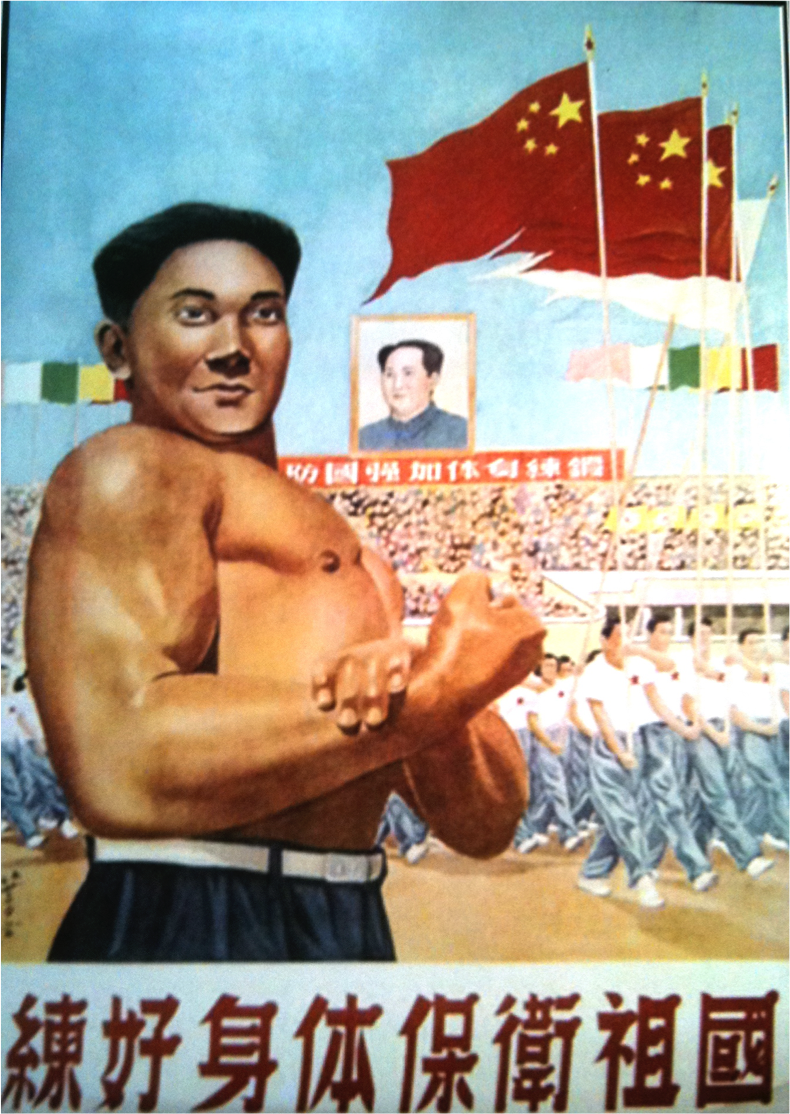
\includegraphics[width = \linewidth]{images/motherlandStrength.png}
  \caption{Strengthen Physique to Defend Motherland (1950)}
  \label{fig:motherlandStrength}
\end{figure}

During this period, China's urban elite began to embrace a range of Anglo-American competitive sports that were promoted by Western missionaries, in particular the YMCA (Young Men's Christian Association).  The YMCA's mission of prescribing Christian manhood for an emerging Chinese youth, including the propagation values of fair play, sportsmanship, masculinity and internationalism, gelled with the values of a nationally (and internationally) motivated urban elite \citep[240]{Morris2004}.  A significant aspect of competitive sports was the fact that they provided a public spectacle, in the form of ``games meets'' (\textit{yundonghui}), in which the performance of emerging national and international political identities could take place \citep{Brownell2008}.
As early as 1908, the Chinese sport community enshrined the Modern Olympic Games as the pinnacle of participation in an international community of nations, and as such, the quadrennial global ritual has since preoccupied Chinese sporting consciousness, and Chinese national consciousness more broadly \cites{Jarvie2008}{Barme2009}[19]{Brownell2008}[3]{Morris2004}{Xu2010}.


\subsection{Rugby in China}
Rugby has been a professional sport in China for seven years (in the form of the Olympic event rugby sevens), before which it had existed as a non-professional university sport for 20 years, first established in 1990 at the Chinese Agricultural University, Beijing. Rugby is part of a large collection of ``cold-gate'' sports (\textit{lengmen xiangmu}, a term that refers to a profession, trade or branch of learning that receives little attention) in China, with a relatively small participation base compared to other interactive team sports like basketball or football.  However, due to the persistent Olympic focus of the Soviet-modelled Chinese competitive professional sports system (\textit{juguo tizhi}), rugby's recently acquired Olympic status (announced in 2009) in the form of rugby sevens means that it has now been inducted into the state-sponsored competitive sports system and is one of 33 sports featured in the all important quadrennial National Games.  Ten of China's collection of 32 provinces and municipalities that participate in the National Games have full time men's and women's rugby programs.

While football and basketball have matured as standalone market-based professional industries, most other sports in China (i.e., all other Olympic events, including rugby) exist primarily due to the support of the enormous state-sponsored national provincial sport system.  Whereas the commercial basketball and football industries might offer a small percentage of prospective athletes incentives of fame and fortune, the benefits of a state-sponsored sports programs like rugby are more modest.  Chinese youth either gravitate or are ushered by their parents towards  sporting careers primarily due to potential life-course opportunities such as access to tertiary education and post-athletic career employment (in the government sports system).  The extent to which an athlete is able to maximise these potential benefits depends on the strength of an athlete's results (\textit{chengji}).
In Olympic sports, the most important measure of a province's success in state-sponsored sporting terms is the National Games, a quadrennial multi-sport event hosted on rotation by provincial capital cities \citep{Hong2002}.  The amount of funding a province and its provincial sporting institutes and programs receive is decided to a large extent by results at the national games.

\subsection{A turbulent history of ``fair play'' in China}
When rugby union became an Olympic sport in 2009, and subsequently inducted into the state sponsored sports system in 2010 (to be played at the national games in 2013), a few provinces in particular identified a potential opportunity to achieve a beneficial National Games result by heavily investing in this debutant sport.  Beijing's Xiannongtan Sports institute managed to attract a large amount of China's existing rugby talent—---including the unofficially touted ``Emperor'' (\citep{huangdi}) of Chinese rugby, national coach Zheng Hongjun—--from where they were previously based at the Chinese Agricultural University, Beijing.  Meanwhile, Shandong province—--a powerhouse in other provincial sports--—succeeded in attracting the majority of the remaining talent, by token of the fact that a large majority of rugby players in China at the time (indeed, a large proportion of athletes more generally) were of Shandong origin.  Importantly, this talent included the Emperor's student come rival coach Lu Xiaohui.  Besides Beijing and Shandong, Jiangsu and Anhui province were strong contenders for the women's gold medal, while the People's Liberation Army (PLA) and Hong Kong in particular were strong contenders for top spot in the men's competition.

Beijing's results leading into the 2013 national games were strongest overall across the men's and women's teams, however the Hong Kong men's and women's teams had only occasionally participated in these tournaments.  In the semi-finals of the National Games, the Beijing men came up against Hong Kong, while the Shandong men played off against the PLA.  Beijing lost to their stronger and more favoured opponents, whereas Shandong beat the PLA.  Meanwhile in the women's league, both Beijing and Shandong advanced to the final.  The stage was set: Beijing, the favourites led by the reigning Emperor of Chinese rugby, would face Shandong, the underdogs lead by the Emperor's cunning apprentice.

The men's final was played first, and in somewhat of an upset, Shandong edged out Hong Kong to win the gold medal by one try.  In the women's final, scores were level until early in the 2nd half when Shandong went ahead by two tries to nil.  At that point, the Beijing women's team, under instruction from their coach Zheng Hongjun, suddenly stopped playing.  After being asked by the referee and match officials to continue, the Beijing women stood firm and refused to play on, forming a huddle on their side of half-way in the middle of the field. Shandong had no choice but to continue to play out the rest of the 2nd half, running in try after try, until the final score at full time was an incredible 71-0.  Shandong was declared victorious, while Beijing called foul play, claiming that the referee had been unfairly adjudicating the match in Shandong's favour.  The details and dramas of this now well-known story in China's sporting history (known as ``Match-striking-gate'') require more detailed development in a format that exists beyond the scope of this particular study.  However, there are two important implications of this incident for my research.

The first implication is the impact this incident had on the Beijing rugby program at Xiannongtan.  The Beijing women's rugby team was the first Beijing team in the 48-year history of the National Games not to receive the ``medal for civilised spirit''  (awarded by the Beijing Mayor to all Beijing representatives in the National Games).  All rugby coaches and many senior athletes of the 2013 National Games campaign have since left XNT: either retiring or moving to other provinces.  The rugby program was all but abandoned in 2014, and finally at the end of 2014 the men's program was resurrected by the appointment of a new head coach Zhu Peihou (a former Agricultural University Coach) and assistant Coach Shiyan.  The women's program was only formally re-established at the end of 2015, with the appointment of former Beijing women's rugby representative athlete Ma Jiale as head coach, and former Beijing men's rugby representative athlete Wang Chongyi as assistant coach.  Rugby is still part of XNT, but is no longer centre stage, and is a shadow of its former glory.  It was in this context that I entered XNT and conducted ethnographic research.

The second implication of this incident is what it says about the ethics of group membership in China.  This is not the first match-striking incident of Chinese sport. In fact, match-striking features periodically throughout recent Chinese sporting history.  In July 2015 Chinese ping pong athlete Zhang Weike failed to turn up to the 9th Round of the ping pong league because in protest at his club's refusal to sign a competition bonus agreement with him for that particular round of competition. The club were holding off signing the agreement because due to Zhang's recent poor form.  In 2004, Beijing Moderns Football Team famously stopped playing mid game against Shenyang Jinde Football Team due to objections with the referee's decisions. It was later revealed in an extensive expose of Chinese football in 2009 that the referee had in fact been bribed to fix the match (along with many other matches during that period), and this incident and many other like it were linked to the control of professional football in China by mafia-run betting rings.

The relevance of this incident to the present study is the fact that match-striking—--a strategy that appears to publicly disregard the sanctity of ``sporting contest''---exists as a viable strategy in the Chinese sporting world. That this option and others make up the behavioural arsenal of athletes, coaches, and officials in competitive sport in China is first an indication that sport in China suffers from a general lack of trust in the values and institutions of fair play, sportsmanship, and the sporting contest that are often celebrated in Western democracies to be the foundational pillars of sport and worthy of fierce deontological defence in and of themselves\citep{Morris2004,Gold2002,Yuki2005}.
There have been various concerted attempts throughout China's modern history to instil the importance of ``fair play'' in Chinese sport \citep{Morris2004,Brownell1995,Brownell2008}, and yet, however intensely politicians, sports officials, coaches, and athletes emphasise in official public rhetoric the importance of such categorical ideals in sport, it is also clear that the behaviour of these very same agents is often heavily determined by networks of power (\textit{quanli}) and interest (\textit{liyi}) that function externally to official institutions and threaten the exact values that are publicly promoted.

%%%%%
China's modern history has been turbulent, tragic, and continually in flux, and sport forms part of this greater story.  While a full dealing with sport in China is beyond the parameters of this dissertation, it is interesting to note that, from a cultural-psychological perspective, interactive team sports in particular have proven far from a ``snug fit'' for China.  Save for occasional flashes of glory in women's volleyball (Gold Medalists at Los Angeles Olympics in 1980), China's team sports have traditionally underperformed on the International stage, to the great embarrassment of the nation \citep{Brownell2008}.  This national embarrassment is most intensely felt in relation to the Chinese men's football team, who often record defeats to minnow neighbouring countries such as Thailand and Hong Kong. When asking my research subjects about the China's team sport issue, a series of physiological and psychological reductions are offered for Chinese peoples' deficiency in the cooperation requirements of team sports: China's one child policy, a culturally-instituted deference to authority and lack of creativity, and a conviction that that Chinese society is too complex and Machiavellian to support pure commitment to the team.  How is it possible to assess these discursive explanations in light of cognitive and evolutionary mechanisms of cultural transmission and social cohesion?

The extent to which cultural psychological processes support and help reproduce the specific socio-ecological phenomenon of sport in contemporary China should also be carefully considered \citep{Sperber1996,Nisbett2003}.  On this level of analysis, the prevalence of scandal and corruption in Chinese sport is perhaps symptomatic of a complex ecology of cultural practices structured by both relational and categorical psychological tendencies relating to social interaction, group formation, and cultural institutions \citep{Nisbett2003,Yuki2005,Liu2009}.\footnote{Indeed, the naivety with which Western countries appear to maintain faith in the sanctity of sport as a pure space for the cultivation and display of virtue and mutual respect, despite obvious evidence to the contrary (use of performance enhancing drugs, match-fixing scandals, exploitation of athletes, etc.) should also be called into question \citep{Southall2017}.  Unfortunately a proper investigation of these questions lie outside the bounds of this dissertation.} What makes group exercise so fascinating is the way in which the culturally-specific patterns and signatures of these complex psychosocial processes can be witnessed at once in the most macro-scale of institutional organisation, right through to the most subtle movement tendency in joint action on the field.


%It is important to approach a study of joint action and social bonding between Chinese professional rugby players with this cultural-psychological variation in mind.
%While the cognitive processes of joint action and social may exist as hypothesised, they may come packaged in  discourses and behavioural tendencies shaped by the specific cultural context.


\subsection{Joint action, team click and social bonding in China}
As mentioned above, while there is very little empirical evidence linking movement coordination and social bonding within the Chinese cultural context, there is extensive indirect evidence from historical and contemporary literatures to suggest ways in which this relationship---between (joint) action and social processes of group formation and cohesion---is uniquely articulated in the Chinese context \citep{Weed2011}.  Historical evidence also suggests that the dynamics of joint action in particular have the focus of ethical considerations, namely resolution of social tensions inherent in collective action problems \citep{Slingerland2014}.

It is well documented that the most prominent metaphor in Chinese cultural discourse is that of the family \citep{Maehr1980}, and that this metaphor structures many extra-kin social relationships between individuals, and between the individual and the state \citep{Gold2002}.  Traditionally, the father-son kinship relationship is utilised to naturalise the socially constructed relationship between lord and minister: ``Parents naturally love their children, and children naturally love and respect their parents, and they both know that they're stuck with one another no matter what...'' \citep[178]{Slingerland2014}. Likewise, the metaphor of family is often utilised to naturalise the notion of an extra-kin social group, for example a company or a sporting team \citep{Brownell2008}.
It is important to emphasise that, whereas traditionally Western (Anglo-American) notions of group membership generally hinge upon a psychological representation of egalitarian equivalence between categories of self and group, the utilisation of the family metaphor for group processes relies on the individual identifying group membership through a participation in hierarchically structured (familial-like) \textit{relationships} \citep{Fei1992}.

It is within these processes of extending familial metaphors to formal social relationships that Slingerland (2014) locates a key role for joint action. Inherent in the scaling up of familial relationships to extra-kin social relationships is the tension common to many collective action problems, that of vulnerability to free-riding and defection \citep{Cosmides2013,Gavrilets2015}.
As Slingerland explains, the ``logic of civilised life makes us very keen to distinguish reliable cooperators from unreliable defectors...what we want then is a particular type of desirable...behaviour where there is absolutely no gap between action and motivation'' \citep[192]{Slingerland2014}. The paradoxical Chinese idiom of \textit{wei wuwei}, translated awkwardly into English as ``trying not to try'' or ``effortless action,'' is promoted in many ancient Chinese philosophical corpuses as a behavioural solution to conflicting incentives involved in coordination problems: effortlessness in performing socially desirable actions (virtues) communicates a level of mutual trust and commitment that is ``hard-to-fake.''  The phenomenology of effortless action is described at length in many of these corpuses, and is a key dimension of many traditional Chinese martial arts such as Taichi and Wushu \citep{Morris1998}.
While mass participation in Anglo-American competitive sports is only a recent phenomenon in China \citep{Brownell2008}, the social valorisation of certain types and styles of movement, particularly the phenomenology of flow in (joint) action appears to enjoy a long history.


\subsection{Modes of group membership and self-construal}
An analysis of literature concerning the cultural psychology of self-construal can provide important insights into the way in which macro cultural processes interact with micro-dynamics of social interaction to structure and constrain cognitive processes implicated with joint action, team click, and social bonding.  As Anthropologists have emphasised for some time \citep{Strodtbeck1961,Kluckhohn1961,Mead1967,Fei1992}, and as cultural psychologists are now beginning to demonstrate in experimental paradigms, processes of group membership appear to vary cross-culturally \citep{Markus1991,Nisbett2001}.  Based on recent cross-cultural research, social and cultural psychologists have developed a theoretical spectrum of group membership processes, the two poles of which can be described as categorical and relational \citep{Hofstede1980,Brewer2007}.  Whereas some cultures, traditionally ``Western'' cultures such as the US, the core of self-definition is based on individual autonomy and separation from others.
The self-concept of relational societies, traditionally understood to be predominantly East Asian cultures, by contrast, is defined primarily based on social embeddedness and interdependence with others comprising their in-groups\citep{Leung2012}.

Unsurprisingly, much of Anglo-American social psychology of the 20th Century is rooted in a categorical mode of representing and measuring group membership.  The canonical self-categorisation paradigm of social psychology \citep{Turner1987}, for example, requires that a bounded individual (experimental subject) make an identification between abstract categories of the self and the in-group or out-group.  Categorical group membership is thus achieved when the perceived differences between the self and other in-group members are smaller than the differences between in-group and out-group members \citep{Yuki2014}.  In distinction to a categorical mode of group membership, relational group membership involves attention to maintaining and harmonising intragroup relationships, engaging in intergroup categorical comparisons \citep{Yuki2003}.
In a relational mode, social identity is less a function of distance between abstract categories of self and in-group, and more a degree of commitment to cultivating a network of hierarchically structured---but more or less self-centred and self-enhancing---network of relationships \citep{Liu2009,Nisbett2003}.

These two predominant modes of group membership—--categorical and relational—--have been shown to vary across cultures (i.e. East Asian versus Western European or North American, see \citep{Markus1991,Nisbett2001,Yuki2003}, within groups (according to sex and personality differences \citep{Yuki2014}, and indeed, within individuals (depending on contextual and situational primes, \citep{Lee2014,Wong2005}).  While the durable persistence of cultural and linguistic institutions appear to be responsible for the prominence of one mode of membership over another (East versus West, for example), recently researchers have suggested that divergent modes of group membership—categorical and relational—may be mediated by context-specific socio-ecological factors such as the level of relational mobility in any given environment \citep{Oishi2010,Takagishi2014,Yuki2005}.  Both modes of group membership have been shown to shape attention, cognition, and behaviour \citep{Nisbett2003} and as such have important implications for the task of identifying and measuring social bonding mechanisms of joint action

Experimental evidence suggests that categorical group processes facilitate fast and effective identification with arbitrary minimal groups \citep{Diehl1990,VanBavel2014}, the arousal of intrapersonal cognitive dissonance between the self and experimentally constructed in-group \citep{Festinger1957, Stone2001}, higher levels of cooperation with categorically similar strangers in economic games \citep{Yuki2005,Yuki2003}, and greater attention to and memory recall \citep{Buchan2006,Ng2016}.  In cultural environments where relational processes of group membership are more prominent or salient, on the other hand, the inverse is usually observed. First, minimal group paradigms have had very little (if any) success in East Asian (particularly Japanese) contexts \citep{Liu2009}.  Relational group processes, on the other hand, allow for the arousal of cognitive dissonance only when it is constructed interpersonally (as opposed to intrapersonally) between an individual and specific individuals to which that individual is connected by a meaningful social relationships \citep{Hoshino-Browne2005}.  Likewise, individuals with a predominantly relational group awareness are more willing to cooperate with and attend to strangers with whom they share relational rather than categorical ties \citep{Ng2016,Yuki2005}.

Relational group membership has a long history in China, rooted in Confucian \citep{Hwang1999}, folk-cultural axioms \citep{Wang2009}, agricultural modes of production \citep{Talhelm2014,Fei1992}, dynastic rule, and modern reinventions of these cultural forms by processes of the nation-state\citep{Liu2014}. The metaphor of the family is particularly salient and pervasive in modern public representations.  On almost every scale of social organisation, from dyadic extra-kin friendships through to workplace interactions and macro-social organisations (cities, provinces, nation), the family and its relational priorities are consistently invoked to aid coordination and coerce participation in collection action.
In addition, the last 150 years of Chinese modern history has also entailed the introduction of categorical group processes associated with the activities of the nation-state, leading to a contemporary Chinese indigenous psychology in which a relational mode is predominant, and a categorical mode is contextually-activated, especially when categories such as ``China'' are threatened or challenged internationally \citep{Liu2009}.

\subsection{Implications for the present study}
The literature reviewed above potentially poses an interesting challenge to the way in which social bonding is understood within cognitive and evolutionary anthropology.  The professional Chinese rugby players that form the focus of this dissertation are young men and women predominantly from rural areas of China's northeast, and are therefore likely subject to relational modes of group membership made predominant and durable by persistent cultural and linguistic processes associated with group membership in contemporary China \citep{Liu2009}.  In addition, athletes are members of a relatively small and stable team environment, for which access to benefits should require attention to the maintenance of productive intragroup relationships, more so than processes of intergroup mobility or comparison \citep{Schug2010}, even though intergroup comparison is an inherent component of competitive interactional team sport. However, given the fact that rugby is an imported team-based interactive sport, for which categorical modes of group membership are required and celebrated, I also expect athletes to exhibit a categorical mode of group membership.
In addition, I expect the metaphors of family to be prominent in the scaffolding of team processes, and I also expect to find a tension between loyalties to the team, and loyalties to an athlete's pre-existing relational networks of family and friends\citep{Yang1994}.  Thus, the specific cultural setting is such that I do not necessarily expect to encounter the type of public representation or testimony of group membership common in Western sporting parlance, more indigenous to the rugby pitches and boathouses of Oxford or any high school American Football movie produced in the 1990s.  Instead, I expect to find evidence of a link between joint action, team click, and social bonding expressed and embodied in cultural representations that may vary distinctly in structure and content from Western intuitions based on a predominantly categorical mode of social cognition.

\section{The Beijing provincial men's rugby team}
I focus my ethnography on the Beijing provincial men's rugby team ($n=26, avg. age=21.3, range = 17-27, SD = 2.96$).  The Beijing provincial men's and women's rugby programs are based at the Xiannongtan Sports Institute in Beijing (one of Beijing's four major sports institutes, and home to seven different full-time sports programs, hereafter Xiannongtan).  These athletes represent Beijing at a provincial level, playing against other provinces in annual tournaments, and every four years at the all-important National Games.  Five athletes have previously represented China in international rugby sevens tournaments.  There is also a Beijing women's rugby team at Xiannongtan, but I was not able to accompany the activities of both teams closely enough to perform adequate ethnographic research.

Members of the Beijing men's rugby sevens team are either already-contracted (n=13) or aspiring professional athletes (n=13) who live and train 6 days a week at Xiannongtan and occasionally attend university or high school classes as part of their ongoing education---what can only be termed part-time education.  A head coach and assistant coach look after the day to day organisation of team schedules and training, and these two coaches are assisted by a further two player-coaches, who are in the gradual process of moving from athlete to coach status.  One of Xiannongtan's four principals is responsible for the management and administration of the rugby program, and is occasionally present at team meetings and national competitions.

Athletes are all from relatively modest socio-economic backgrounds, many hailing from suburban and rural areas of northern China (Shandong (11), Beijing (6), Jiangsu (3), Liaoning (2), Hebei (2), Anhui (1), Henan (1), Heilongjiang (1)).  The squad consists of 10 fully contracted senior athletes (\textit{xieyi}), three provisionally-contracted athletes \textit{shixun}, and six student-athletes \textit{erjiban} who do not receive a salary but receive training, food, board, and educational support.  The remaining athletes (7) are classed as athletes in training \textit{jixun} and are effectively on trial until they either show promise or withdraw from the squad either voluntarily or upon suggestion by the head coach.  Provided that they meet the relevant academic and athletic requirements, contracted and student athletes are able to attend the Beijing Sports University—considered to be the country's most prestigious sports university and one of China's ``top brand universities'' (\textit{mingpai daxue}).

The average rugby training age (years spent playing rugby) of Beijing athletes is 3.12 years ($range = 0.16 – 10 years$).  Contracted senior athletes ($average age = 24.3 years$) have trained for an average of 5.4 years, whereas the average training age of junior non-contracted athletes (average age = 19.3 years) was 1.7 years.  Over half of the athletes have a background in other sports (15 athletes from track and field, one from football, one from basketball), usually beginning part-time or full-time physical training at the age of 11-13.  Those who transferred to rugby did so either at the beginning of senior high school (16 years) or at university age (18yrs).  The rest of the group had no particular sporting background before starting at Xiannongtan, and were scouted by school athletics coaches based on their basic athletic attributes (running speed, strength, coordination, and potential for physical growth).  Of the 26 athletes in the squad, three junior athletes who were part of the squad when I arrived in September 2015 have now left, and three new athletes have arrived. This movement of non-contracted players in and out for trials is quite common.

\subsubsection{Training schedule}
Every year between April and September there are five national tournaments held in different locations across the country.  October –-- February constitutes the off- and pre-seasons for these yearly competitions, during which time teams travel to domestic or international training locations depending on amount of program funding and training strategy.  In 2015, before an unexpected change in coaching team at the end of December, plans were to travel to Yunnan in the new year province for altitude training (January) before moving to sea-level somewhere in the south (February/March).  Following the coaching leadership change, the team did not leave Beijing until after Chinese New Year (15th February), which meant that training during this period was influenced by Beijing's cold winter weather and air pollution.

Below is a table of a typical weekly training schedule. A typical week consists of 10x2.5hr training sessions, three of which are strength and conditioning sessions, seven of which are on-field rugby sessions.  In addition, two one hour evening skills sessions are also added for junior athletes to hone their basic skills of passing, catching, and game-play.  Athletes live full-time on campus at XNT in dormitory accommodation (usually 3 athletes per ensuite room), and are permitted leave on the weekend after the conclusion of Saturday morning training.  Athletes with family in Beijing usually take this leave, while the remaining athletes spend weekends at XNT.  Athletes break at the end of season (September) for two weeks, and occasionally around Chinese New Year for 7-10 days, unless New Year interrupts pre-season training plans, in which case training continues throughout.


\begin{table}[htpb]\caption{Weekly Training Schedule}
  \begin{center}
    \begin{small}
        \begin{tabular}{| c | c | c | c | c | c | c | c |}
          \hline
          & \bf M & \bf T & \bf W & \bf T & \bf F & \bf S & \bf S \\
          \hline
          0600 & Training &  &  & & & & \\
          \hline
          0900 &  & Training & Training & Training & Training & Training &  \\
            \hline
          1500 & Training & Training & & Training & Training & Training &  \\
            \hline
          1900 &  & Training (junior athletes) & & Training (junior athletes) & & & \\
             \hline
        \end{tabular}
      \end{small}
    \end{center}
  \end{table}


\section{Research methods}
Ethnographic data included: unstructured and semi-structured interviews with athletes and coaches (yet to be analysed in-depth), general and activity-specific surveys, and field notes based on participant observation of daily activities of the team.


\subsubsection{Participant observation}
For 6 months in 2015-16 and 6 weeks in summer 2016, I lived and trained full time with the team at XNT, during which time I took daily field notes using a note taking application (Evernote, version 6.11), which was synced between my mobile phone and personal computer. I collated, summarised, and tagged these notes weekly or fortnightly.

\subsubsection{Interviews}
In addition to ad-hoc unstructured interviews with athletes, coaches, and other officials XNT officials and individuals in the Chinese rugby community (n = 15), I conducted 26 semi-structured interviews, each lasting between 15 and 70 minutes.  All interviews were conducted in Modern Standard Chinese (Mandarin) and were recorded with participant consent using a sound recording application on my smartphone or laptop computer.

During semi-structured interviews, I asked athletes about their personal background (including their family situation), their motivations for adherence to rugby, perceived costs and benefits of adherence to rugby, their perceptions of role in the team, their experience of playing rugby (particularly feelings of flow, dissonance, and team click).  The structured interviews also involved two tasks, one in which the athlete was required to rank motivations for adherence to rugby, and one in which the athlete was asked to report their three closest friends in the team, the three team members most willing to sacrifice on behalf of the team, and three most competent athletes in the team (see Appendix for full script). Athletes answered these questions using a pen and paper. I later collated and uploaded these responses to Evernote.


\subsubsection{Surveys}
 I conducted a number of informal surveys designed to understand athletes' general and specific experiences group membership.  I conducted surveys following three training sessions: a session in which athletes (predominantly junior athletes) ran an aerobic fitness test involving straight-line running shuttle-running at and above the aerobic threshold (Beep Test), and two training sessions involving internal game-like scenarios.  In addition, I asked athletes about their general experiences of team membership agency over the team (weak-strong), role in the team (central-marginal), individual performance (weak-strong), team performance (weak-strong), training intensity (\textit{qiangdu})(light-heavy) at two three-month intervals.
